\section{Animación de la anatomía humana} 
\label{art:anatomy}


%\subsection{Introducción}

Una de las necesidades básicas que debe cubrir un simulador es poder mostrar información anatómica de pacientes virtuales con la que trabajará el usuario. En  \cite{preim2018survey} se explica la necesidad de que los estudiantes tengan un conocimiento profundo de la anatomía humana, estructuras, su posición relativa, variabilidad, etcétera. Es fundamental que un médico cuente con esos conocimientos previamente a la realización del entrenamiento médico.

Existen dos formas comúnmente utilizadas para representar modelos tridimensionales por computador. Tradicionalmente, se utiliza una malla compuesta por facetas poligonales 2D (triángulos o rectángulos) que representa solo la superficie o contorno del modelo sin tener en cuenta ninguna información interna. Estas representaciones se llaman comúnmente \acp{B-rep}. En el momento de \emph{renderizar} se proyecta la geometría y se calcula su iluminación sin interaccionar con el interior del modelo.
% Lo más habitual es utilizar una malla poligonal que define la superficie o contorno del modelo que se representa. Estas mallas están normalmente compuesta por triángulos o rectángulos (quads), comúnmente llamadas \ac{B-rep}. Estas mallas son utilizadas para representar solo la superficie del modelo sin tener en cuenta ninguna información interna.  % \del{Esta malla generalmente está compuesta de polígonos llamados facetas o caras que son la unidad básica de un modelo tridimensional. Las caras más comunes son: triángulos, siendo este el polígono más simple; o rectángulos, que normalmente se descomponen en dos triángulos. El triángulo es la figura más utilizada debido a su menor complejidad matemática en los diferentes cálculos relacionados con la informática gráfica (interpolaciones, manejo de vecinos, etc.).}
%A lo largo del tiempo, las tarjetas gráficas se han diseñado con especial énfasis en el tratamiento de triángulos.
%Por otra parte, existe otro tipo de representación, llamada volumétrica, que permite una representación visual completa de un objeto tanto del exterior como del interior, que la representación poligonal no era capaz. Sin embargo, esto produce una gran complejidad al intentarlas \emph{renderizar} mediante técnicas de imagen generada por computador.

Por el contrario, 
existe otro tipo de representaciones  llamadas volumétricas. Los objetos volumétricos pueden ser representados como una pila de imágenes 2D (\emph{stack} de imágenes), mallas de poliedros, o una imagen  tridimensional formada por \emph{vóxeles}\footnote{Unidad cúbica mínima para representaciones volumétricas.}. A la hora de \emph{renderizar} estas representaciones, existen una variedad de técnicas más complejas (p. ej. técnica \emph{ray casting} \cite{isabel}) para \emph{renderizar} modelos volumétricos.


En la figura \ref{fig:HVP} se puede apreciar dos \emph{renderizados} del mismo modelo anatómico.

\begin{figure}[ht]
   \centering
    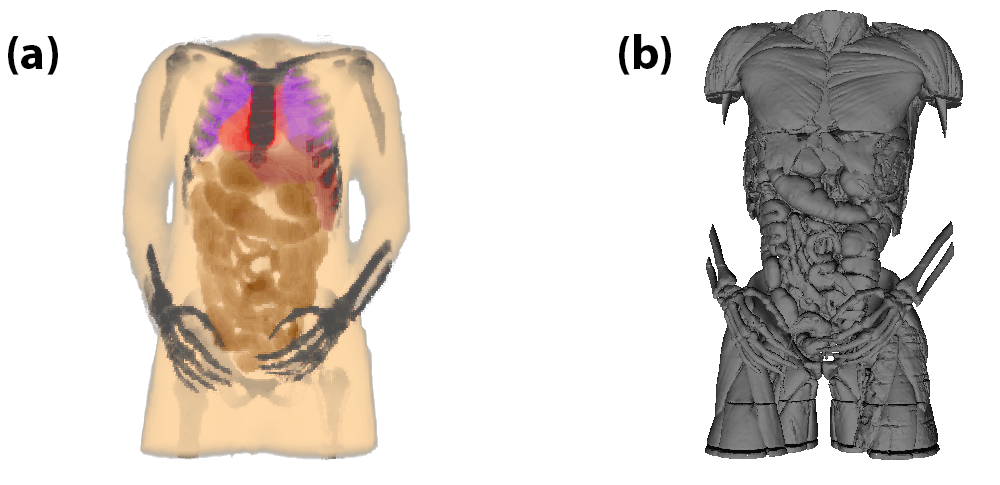
\includegraphics[width=0.9\textwidth]{IMG/volvsb-rep.png}
    \caption{La figura (a) muestra el \emph{renderizado} de la representación volumétrica del \emph{Visible Human Project} \cite{ackerman1998visible} mediante \emph{Ray-casting}. La figura (b) muestra el renderizado de la malla poligonal del mismo modelo. }
   \label{fig:HVP}
\end{figure}
%\todo{hace falta explciar la malla de tetraedros?}



Respecto a la representación de modelos anatómicos humanos, es fácil encontrar  varios modelos comerciales como pueden ser: \emph{ZygoteBody}$^{TM}$ \cite{kelc2012zygote}, \emph{Anatomium} \cite{Anatomium}, \emph{BioDigital Human} \cite{qualter2012biodigital} o modelos como \emph{Visible body} \cite{visible2012visible} que solo está centrado en músculos y dispone de una serie de animaciones predefinidas. Todos ellos representados como mallas de polígonos. Estos modelos han sido diseñados por artistas y representan cánones no realistas, además no reflejan fielmente la variabilidad anatómica de los pacientes a la que podría enfrentarse un médico. En ocasiones, estos modelos no están diseñados correctamente al presentar intersecciones y colisiones entre tejidos como se puede observar en el Entregable 3.2 del proyecto \ac{RASimAs} titulado \emph{Patient-Specific Dataset Library} \cite{ded3.2}.

En la actualidad, existe una línea de investigación muy activa para transferir datos de pacientes reales a modelos virtuales y de esta forma usar datos capturados a partir de diferentes técnicas de imagen médica (como \ac{TC}, \ac{IRM} o \ac{US}). La base de datos de  \emph{Visible Human Project} \cite{ackerman1998visible} y  \emph{Segmented Inner Organs} \cite{VoxelMan} basado en el anterior, representa uno de los modelos volumétricos de prueba más utilizado en la búsqueda de métodos para extraer modelos virtuales procedentes de imágenes médicas \cite{ferrante2017slice}.

Tanto los modelos comerciales como los modelos obtenidos a través de imagen médica muestran el mismo problema: los modelos anatómicos son presentados en una misma postura, que suele coincidir con la postura de adquisición. Esto hace que los datos de pacientes sean estáticos y, por consiguiente, no permiten adaptarse a la posición requerida. Algunos procedimientos médicos, como la artroscopia de rodilla o el bloqueo del nervio axilar, requieren posturas diferentes a las que se obtuvieron en el momento de la adquisición de la imagen médica. En el caso de la artroscopia, se necesita la rodilla flexionada frente a la habitual imagen capturada de la pierna extendida. En el caso del bloqueo del nervio, es necesario que el paciente se sitúe con el brazo en abducción de 90 grados respecto del tronco y el antebrazo en flexión de 90 grados en comparación a la mayoría de las imágenes médicas que son capturadas en una posición relajada. 

Es importante destacar que la mayoría de las técnicas de imagen médica no son capaces de capturar adecuadamente todos y cada uno de los tejidos del paciente. Por tanto, los métodos de registro entre imágenes médicas y modelos anatómicos tridimensionales que se presentan en \cite{ferrante2017slice} es habitual que se centren solo en tejidos concretos, como pueden ser la piel, huesos y músculos en general. 
En cuanto a las propiedades mecánicas de los tejidos, existen técnicas como la elastrografía \cite{MRIelastography} para recuperar la elasticidad o dureza de un tejido concreto. Aun así, esta técnica no permite la adquisición de la descripción mecánica de todos los tejidos.



%de registro entre imágenes médicas y modelos anatómicos tridimensionales que se presentan en \cite{ferrante2017slice} no son capaces de capturar adecuadamente todos y cada uno de los tejidos del paciente. En ocasiones solo se centran en tejidos concretos como puede ser la piel, huesos y músculos en general. Además, las técnicas actuales de imagen médica tampoco son capaces de recuperar las propiedades mecánicas de todos los tejidos, siendo esto un gran inconveniente si se requiere una descripción de todos los tejidos.

Por tanto, se necesita un método que permita a los simuladores tratar modelos virtuales sin importar la posición con la que fueron creados. % con tejidos internos, completos o incompletos, y poder adaptar su postura al procedimiento a entrenar. Se busca poder utilizar una variabilidad de modelos, con el objetivo de que los usuarios puedan entrenar con el máximo número de pacientes virtuales del que se dispongan 
Por ejemplo, se puede hacer mención al trabajo de  \emph{Dicko et al.}~\cite{Ali2013}.  En este artículo, los autores han desarrollado un método para modelar la anatomía interna de un paciente virtual, transfiriendo los tejidos internos de un modelo anatómico de referencia como \emph{ZygoteBody}$^{TM}$~\cite{kelc2012zygote} a un modelo registrado a partir de una imagen médica. Con esta técnica, es posible registrar y modelar los tejidos internos de datos obtenidos de \ac{IRM}. Este trabajo se centra solo en el proceso de registro y modelado sin detallar el proceso de animación utilizado, en el que no se mencionan como se realiza la etapa de \emph{rigging} o la de pesado, las cuales se detallarán más adelante. Además, se citan ciertos problemas con la interpretación de los tejidos adiposos.   


En la siguiente sección, se presentará una visión general de los diferentes algoritmos existentes para animar modelos tridimensionales de caracteres articulados. La animación consiste en deformar las representaciones superficiales 
%\todo{quieres que utilice el termino b-rep?. Marcos. Solo cuando quede bien}
o volumétricas por medio de modelos matemáticos. Estas técnicas se clasifican en dos grupos: aquellas que tienen en cuenta las propiedades físicas del modelo y aquellas que solo utilizan operaciones geométricas para animar el modelo. Actualmente, es habitual que los algoritmos geométricos estén orientados a aplicaciones interactivas, ofreciendo soluciones plausibles, %ser interactivos
%sacrificando precisión  
frente a los algoritmos físicos centrados en una deformación precisa. Aun así, existen algoritmos que combinan ambos enfoques para conseguir deformaciones más precisas para técnicas interactivas, o reducir el tiempo de cálculo para simular el comportamiento físico. 


\subsection{Animación esqueletal}
\label{art:animation}
\label{art:virtualskel}

La animación esqueletal es un método geométrico que se utiliza para animar un modelo articulado representado por su malla superficial, gracias a un esqueleto virtual, asociando los vértices a los huesos virtuales. %Esta técnica permite transferir el movimiento del esqueleto a la representación superficial. 
Esta técnica fue introducida por N. Magnenat Thalmann en 1988 \cite{thalmann88} y sigue siendo la técnica más utilizada debido a su sencillez y su fácil implementación en el cauce gráfico actual. A pesar de la existencia de métodos más realistas, esta técnica se usa prácticamente en todos los sistemas de animación interactivos ya que simplifica el trabajo de los artistas (el número de grados de libertad del esqueleto virtual es mucho menor al numero de grados de libertad de la representación superficial) o forma parte de algoritmos más complejos como paso previo. %Por ejemplo, se puede animar mediante captura de movimientos y cinemática inversa, entre otros.

La técnica se basa en una abstracción matemática, un esqueleto virtual, que se utiliza para definir los puntos de rotación de las \ac{joints} de los modelos. Este esqueleto se define como un conjunto de huesos virtuales jerarquizados que se encuentran conectados entre sí. La figura \ref{fig:virtualskeleton} muestra un esqueleto virtual superpuesto a un paciente virtual. Las esferas grises representan los centros de rotación de los \emph{\acs{joints}}, mientras que, los prismas representan la relación de herencia entre ellos. Estos huesos están pensados para que el artista dirija los movimientos del personaje y defina animaciones que la técnica de \emph{skinning} trasladará a la malla superficial según se define en \cite{thalmann88}. 

\begin{figure}[ht]
   \centering
    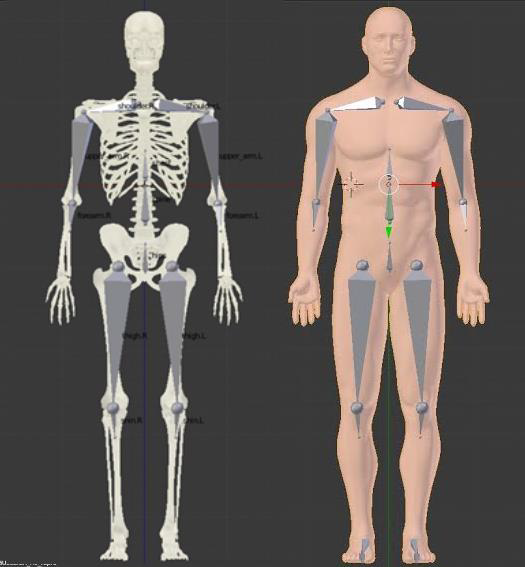
\includegraphics[width=0.8\textwidth]{IMG/virtualskeleton.png}
    \caption{Esqueleto virtual ajustado al tejido óseo de un modelo anatómico.}
   \label{fig:virtualskeleton}
\end{figure}

Con el paso del tiempo, esta técnica ha sido divida en fases que definen el cauce de la animación esqueletal:

\begin{itemize}
    \item \emph{Rigging}\footnote{Término ampliamente utilizado para la creación o adaptación del esqueleto virtual.}: en esta etapa se crea el esqueleto virtual específicamente para el modelo que se vaya a animar.
    \item Pesado: una vez creados los huesos virtuales, se asigna el peso %de influencia 
    de cada hueso para cada vértice de la piel del modelo.
    \item \emph{Skinning}\footnote{Término ampliamente utilizado para la transferencia de movimiento del esqueleto virtual al \emph{\acs{B-rep}}.}: se definen los algoritmos que van a transferir el movimiento de los huesos virtuales a la malla superficial asociada. 
    \item Selección de poses: se define la posición de los huesos que producen una deformación concreta al modelo superficial.
\end{itemize}

A continuación, se mostrará la revisión de la literatura existente para cada etapa, donde se hará especial mención a aquellas técnicas automáticas.


\subsubsection{Rigging}
\label{art:rigging}

El proceso de \emph{rigging} consiste en crear un esqueleto virtual que se adapte a la fisionomía del personaje virtual. Este trabajo normalmente es realizado por un artista ayudado de un programa de \ac{CAD} como puede ser \emph{Blender} \cite{blender} o \emph{3DS MAX} \cite{3ds}. 

Existen algunos trabajos que tratan de automatizar el proceso de creación de esqueletos virtuales siguiendo dos enfoques: generar un esqueleto virtual a partir de la \emph{\ac{B-rep}} o adaptar un esqueleto ya creado al modelo de entrada.

Algunos métodos permiten inferir un esqueleto en base a cualquier malla superficial. A partir de operaciones matemáticas (suavizado Laplaciano en el caso de \cite{laplacian}), se realiza una contracción de la malla que da lugar a un modelo alámbrico. Este será utilizado como esqueleto virtual. Este método presenta la ventaja de poder adaptarse a cualquier modelo no humanoide. Un trabajo más reciente se puede encontrar en \cite{Tagliasacchi}.

En ~\cite{borosan2012rigmesh}, \emph{Borosán et al.} presentan un método que permite modelar y crear el esqueleto virtual en el mismo instante. El artista esboza la silueta y el algoritmo genera la superficie formada por cilindros consecutivos, los cuales son utilizados para crear el esqueleto.


En otras técnicas como \cite{huang2013robust}, se adapta un esqueleto virtual predefinido al modelo de entrada. Normalmente orientado para humanoides, dividen la malla de entrada en segmentos de partes específicas de la anatomía humana (cabeza, piernas, brazos, etcétera) que se utilizan para definir los puntos de rotación de cada hueso virtual. Estas técnicas son más habituales cuando se requiere animar modelos procedentes de una nube de puntos capturados por dispositivos de captura.

En \cite{avril2016animation}, \emph{Avril et al.} se presenta un trabajo en el que, a partir de un personaje virtual de referencia, se puede adaptar el esqueleto y el pesado del modelo seleccionado a cualquier malla humanoide.


\subsubsection{Pesado}
\label{art:pesado}

Este proceso determina cual es la influencia de cada hueso virtual en cada vértice de la malla superficial.
% La consideración de esta influencia se denomina pesado, 
El cálculo de esta influencia se denomina pesado, debido a que se calculan una serie de pesos $w_{i,j}$ que relacionan un vértice $i$ con el hueso $j$.
Para asegurar una deformación correcta, se presuponen las siguientes condiciones:
\begin{eqnarray}
%\begin{equation}
\label{cond1}
w_{i,j}\geq 0 \;\;\;\;\;\;\;\; \forall i \in V \wedge \forall j \in B   \\
%\end{equation}
%\begin{equation}
\label{cond2}
\sum_{j \in B} w_{i,j} = 1\ \;\;\;\;\;\;\;\;\;\;\;\;\;\;\;\;
\forall i \in V
%\end{equation}
\end{eqnarray}
donde $V$ es el conjunto de vértices de la malla poligonal y $B$ es el conjunto de huesos en el esqueleto virtual. No puede existir un hueso que influya negativamente a un vértice, por ello se tiene que cumplir la condición \ref{cond1}. %la relacion no puede ser proporcional añ hueso ao la suma de influencia 
%Ademas, existe (se impone) una segunda condicion, 1.2, que determina la relación de pesos de todo los vertices i pertenecientes a un mismo hueso j y limita los movimientos posibles. 
Además, se debe garantizar que la suma de pesos es proporcional a las influencias de cada hueso, cumpliendo la condición \ref{cond2}.
Por último, resulta intuitivo pensar que las transiciones entre huesos virtuales deberían ser progresivas, el gradiente de los pesos debe ser suave, para evitar efectos extraños y discontinuidades en la malla.

Originalmente, al igual que la etapa anterior, un artista era el encargado de realizar la tarea manualmente, donde se utilizaban herramientas \ac{CAD} para \emph{pintar} la influencia de un hueso en la malla superficial. Actualmente en la literatura se pueden encontrar métodos totalmente automáticos \cite{huang2013robust,pan2017automatic}. 
Algunos de estos trabajos no tienen en cuenta la conectividad de la malla y puede ser que haya vértices topológicamente lejanos con pesos similares. Es por eso, que se han propuesto soluciones como \cite{Baran:2007}, donde se utiliza la ecuación del calor, suponiendo que los pesos se difunden al igual que lo haría la temperatura, permitiendo calcular transiciones más suaves en la malla. \emph{Baran y Popovi\'{c}} resuelven la ecuación en el equilibrio sobre la superficie, añadiendo transferencia de calor en los vértices más cercanos al hueso. El equilibrio en la superficie para el hueso $i$ es dado por:
\begin{equation}
\label{eqn:baran}
 \frac{\delta \mathbf{w_i}}{ \delta t} = \mathbf{ \Delta w_i} + \mathbf{H(p_i-w_i)} = 0,
\end{equation}
donde $\Delta$ es el operador \emph{laplaciano}, $p_i$ es un vector donde $p_{i,j}=1$ si el hueso i más cercano al vértice j, $p_{i,j}=0$ si no lo es, y $\mathbf{H}$ es una matriz diagonal donde $Hjj$ es la contribución del peso del hueso más cercano al vértice $j$.

Aunque esta solución es más compleja (resolución de sistemas de ecuaciones, cálculo de vecindad, etcétera), ofrece transiciones más realistas sin intervención manual. %y menor intervención manual. 
Esta técnica está restringida a mallas superficiales que deben rodear completamente al esqueleto virtual.

Existen trabajos posteriores como el de \emph{Jacobson et al.}~\cite{Jacobson:2011}, donde se mejora la etapa de pesado para ser capaz de manejar puntos de anclaje, huesos virtuales y cajas contenedoras. Se propone minimizar la energía \emph{Laplaciana} de las restricciones de los anclajes con el objetivo de conseguir una continuidad  de primer orden (Ec. \ref{eqn:1}):
\begin{equation}
\label{eqn:1}
\mathrm{arg\,min}_{\mathbf{W_j}, j=1..m}\sum_{j}^m\frac{1}{2}\int_\Omega \left \|  \nabla \mathbf{W_j}\right \|^2 dV,
\end{equation}
donde $W_j$ son los pesos del manejador $j$ y $m$ es el número de puntos de anclaje. La principal limitación es que se genera un problema disperso y cuadrático para imponer las restricciones. %No obstante, en el capítulo \ref{cap:pesado}, la solución propuesta solo requiere resolver un sistema de ecuaciones lineales.

\subsubsection{Skinning}
\label{art:skinning}

Esta etapa es la que define como se transfieren los movimientos de los huesos virtuales a los vértices que componen la malla superficial que los envuelve utilizando la ecuación de \emph{skinning}: 
\begin{equation}
\label{eqn:skinning}
\mathbf{v'_{i}} = \sum_{j \in B} w_{i,j}f(\mathbf{\theta_{j}},\mathbf{v_{i}}) 
\end{equation}
Esta ecuación determina como calcular la nueva posición del vértice $v'_{i}$ de la malla. Donde $\theta$ representa el movimiento de cada hueso $j$ que se aplica a ese vértice. %De esta forma, la nueva posición del vértice se calcula en función de la influencia del movimiento de cada hueso.

Según la formulación matemática que se desarrolle, los distintos métodos toman su nombre, como por ejemplo: \ac{LBS} \cite{thalmann88}, \ac{DQS} \cite{Kavan2008} o \ac{SBS} \cite{Kavan:2005}.



La técnica más habitual es \ac{LBS} presentada en \cite{thalmann88}, que se basa en calcular la nueva posición interpolando linealmente las matrices de transformación $T$ de cada hueso virtual:
\begin{equation}
\label{eqn:LBS}
\mathbf{v'_{i}} = \sum_{j \in B} w_{i,j}\mathbf{T_{j}v_{i}}
\end{equation}

\ac{LBS} sufre problemas debido a que la interpolación de las rotaciones se realiza de manera lineal. Esto lleva asociado efectos no deseados como: el colapso de la malla  en rotaciones (\emph{collapsing elbows}) o en giros (\emph{candy wrapper}). En la literatura, se pueden encontrar numerosas propuestas que solventan los defectos de esta técnica \cite{rumman2016state}, aunque normalmente llevan asociadas un incremento del coste computacional, o la aparición de otros artefactos no deseados. Uno de los métodos más populares es la técnica presentada por \emph{Kavan et al.} en \cite{Kavan2008}, llamada \ac{DQS}, que solventa las limitaciones de \ac{LBS} al utilizar la interpolación de cuaterniones duales (Ec. \ref{eqn:DQS}). Además, esta técnica se caracteriza por ser computacionalmente equivalente a \ac{LBS}. Aunque \ac{DQS} funciona adecuadamente en la mayoría de los casos, en algunas situaciones ocurre que la malla se deforma en exceso. Visualmente, resulta en una ganancia de volumen significativa (\emph{joint-bulging}). 

\begin{equation}
\label{eqn:DQS}
\mathbf{v'_{i}} = (\sum_{j \in B} \mathbf{DQ_{j}}w_{i,j}) \mathbf{v_{i}}
\end{equation}

Otras soluciones se han presentado como en \emph{Lee et al.}~\cite{Lee2013}, donde se describe una técnica que se encarga de resolver los problemas de \ac{DQS} cuando se realizan escalados y cizallados, movimientos muy habituales en cine de animación pero infrecuentes en modelos anatómicos.

En trabajos más recientes, \emph{Le y Hodgins}~\cite{le2016real} presentan una técnica que calcula unos nuevos \ac{COR} para cada vértice de la malla. Este enfoque solventa el problema de \emph{joint-bulging} sin incrementar el coste computacional y no sufre del defecto \emph{candy wrapper}. El único inconveniente es la necesidad de un proceso previo para calcular todos esos nuevos centros.
%\todo{pongo el algoritmo de cor?}
% \begin{eqnarray}
% \label{eqn:COR}
% R = normalize( w_{i,1}q_{1} + w_{i,2}q_{2} + . . . + w_{i,b}q_{b})\\
% t = R_{LBS}c_{i} + t_{LBS} - Rc_{i} \\
% v'_{i} =  R_{q}v_{i} + t
% \end{eqnarray}

%\todo{pongo imágenes de comparación?}
En la figura \ref{fig:corexample} se puede observar una imagen extraída de \cite{le2016real}. En esta figura se muestra una comparativa visual entre su método \ac{COR} y las dos técnicas clásicas más conocidas en la literatura, \ac{LBS} y \ac{DQS}. En cuanto a la rotación del codo, se aprecia que la articulación se colapsa (\emph{collapsing elbows}) en el caso de \ac{LBS}. En su lugar, la técnica \ac{DQS} produce un abultamiento (\emph{joint-bulging effect}), mientras que \ac{COR} resuelve ambos defectos. Respecto a los giros, es conocido que la técnica \ac{DQS} solventa el problema \emph{candy-wrapper} de \ac{LBS}. Se puede observar en las imágenes de la derecha que la técnica \ac{COR} solventa los efectos anteriormente mencionados (\emph{collapsing elbows}, \emph{joint-bulging} y \emph{candy-wrapper}). 

\begin{figure*}[ht]%[b]%[b!ht]
  \centering
  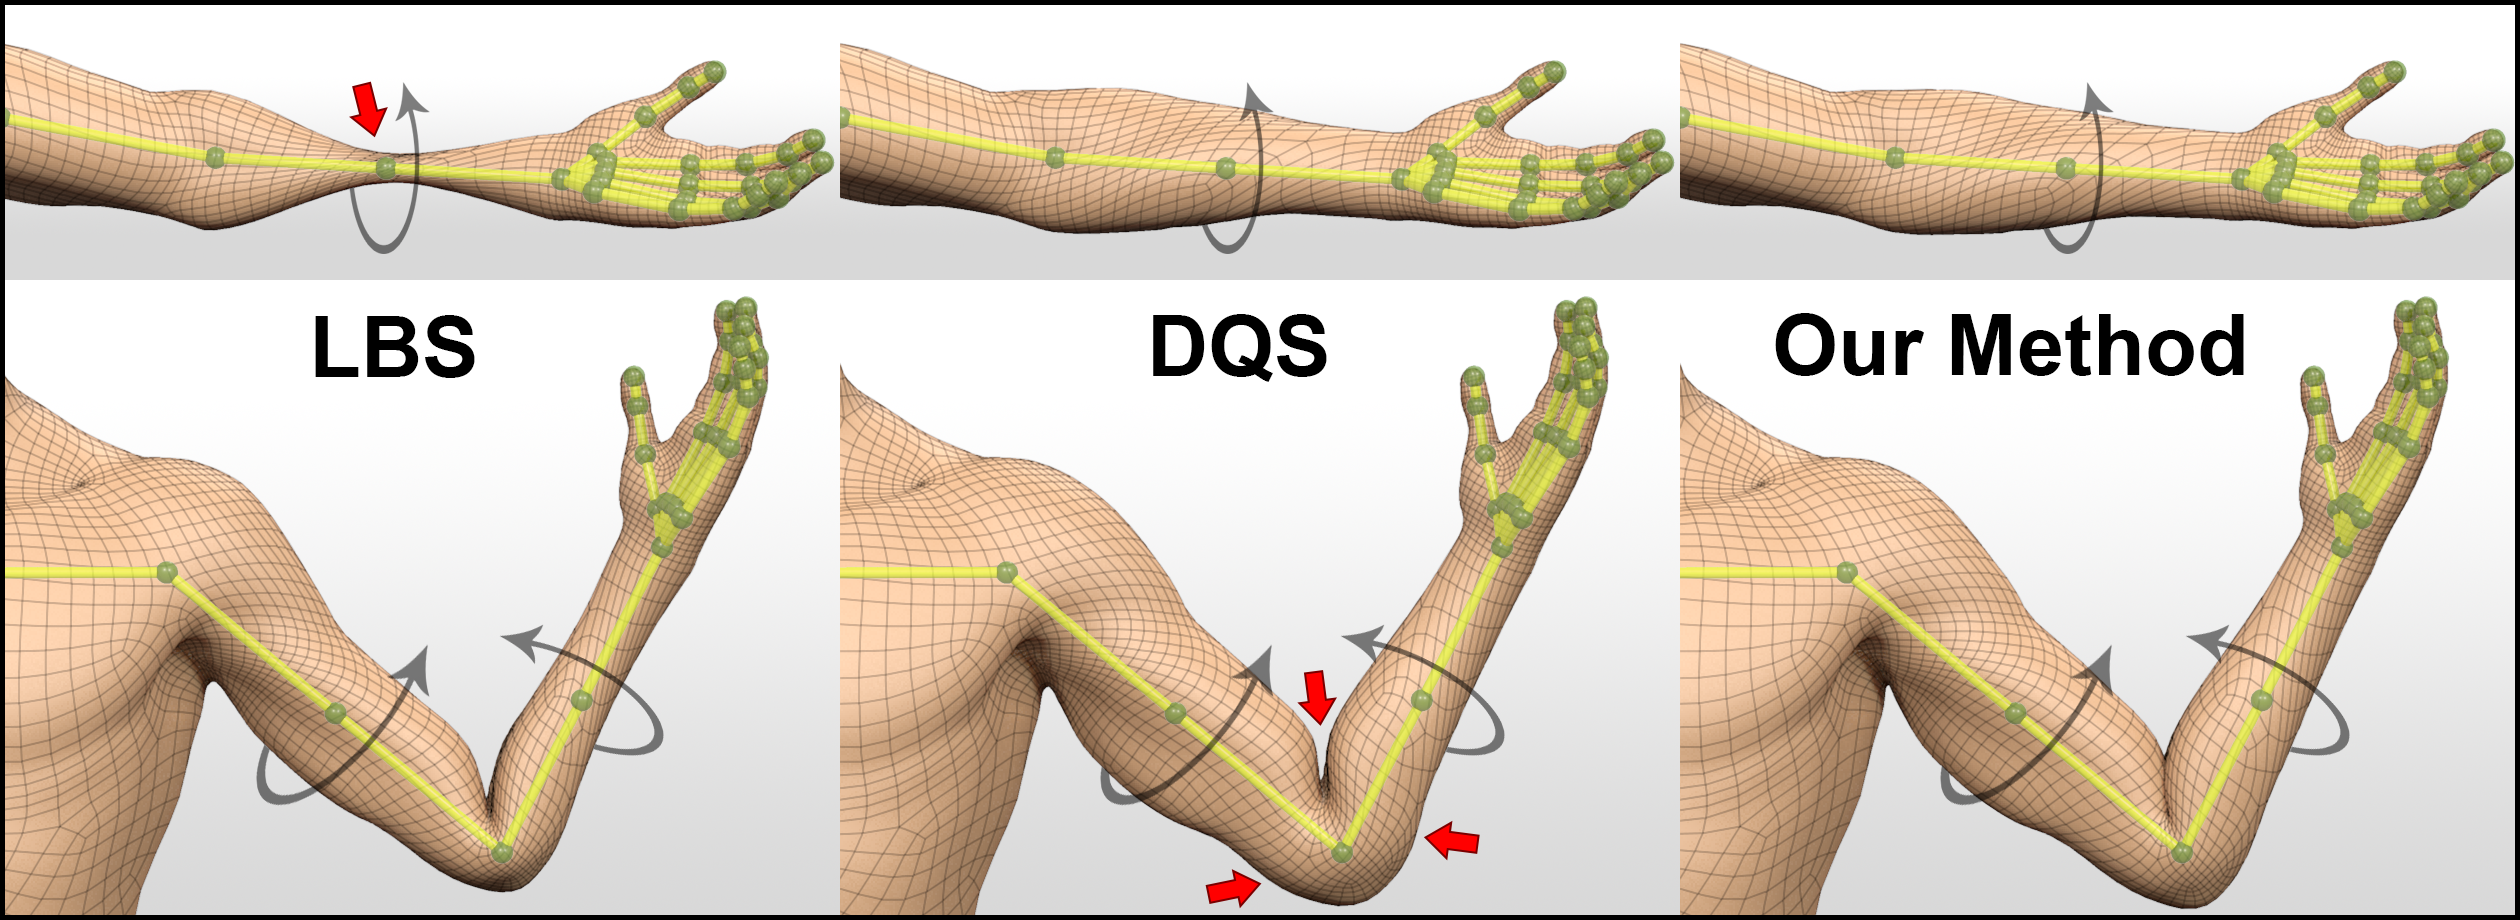
\includegraphics[width=0.90\textwidth]{IMG/corexample.png}
    \caption{En la fila de arriba, se aprecia el comportamiento de las 3 técnicas frente a los giros. \acs{LBS} sufre \emph{candy-wrapper}, mientras las otras dos técnicas no. En la fila de abajo, se puede observar la rotación del codo. En este caso, \acs{LBS} sufre \emph{collapsing elbows}, \acs{DQS} se puede apreciar el efecto \emph{joint-bulging}, y el método \acs{COR} es robusto ante estos defectos. Imagen extraída de \cite{le2016real}. }
    \label{fig:corexample}
\end{figure*}
%%%%%%%%%%%%%%%%%%%%%%%%%%%%%%%%%%%%%
%
%
Otra característica que no es habitual que se tenga en cuenta es la resolución de contactos entre vértices de la malla. En \cite{Vaillant:2014}, se propone una solución geométrica con tasas interactivas que puede solucionar las auto colisiones. \emph{Vaillant et al.} calculan un campo escalar para cada hueso, donde los vértices serán influenciados por el valor de cada campo escalar. Sin embargo, ese método no está pensado para animar modelos que representen tejidos óseos. Estructuras rígidas como los huesos se ven afectados por una función de suavizado, que se traduce en deformaciones no realistas. %16k de vertices 50 fps nosotros 1.5kk

Cuando se trata de animar modelos orgánicos, el uso de esqueletos virtuales, que solo se definen por rotaciones, presenta limitaciones al tener unos movimientos más complejos. Algunos trabajos intentan definir articulaciones basadas en modelos anatómicos \cite{joints} con \emph{splines}\footnote{Curva diferenciable definida en porciones mediante polinomios.}, mejorando así el movimiento del hueso pero dificultando la creación del esqueleto virtual y el proceso de animación.

\subsubsection{Selección de poses} 
\label{art:poses}
Esta etapa consiste en crear las animaciones  y los movimientos de los huesos virtuales que serán aplicadas a la malla superficial.   

Al igual que etapas anteriores, es habitual que estas animaciones sean creadas por artistas profesionales. Con la ayuda de las herramientas \ac{CAD}, los animadores definen el movimiento de los huesos virtuales en fotogramas clave \cite{keyframe}, al igual que se hace en la animación clásica. Una vez definidas las posiciones claves, el software calcula la interpolación de los fotogramas intermedios. Estas herramientas también incluyen algoritmos de cinemática inversa \cite{Shi:2007}, que permiten al usuario posicionar el actuador final (hueso situado en un nivel inferior de la jerarquía) y calcular la posición del resto de articulaciones superiores. 


Existen técnicas diseñadas con objeto de automatizar la fase de animación. Las técnicas de \emph{retargeting}\cite{Choi999} tienen como objetivo transferir los movimientos de un personaje virtual a cualquier otro. Trabajos más recientes no necesitan que los esqueletos virtuales tengan la misma estructura \cite{Hecker2008}, e incluso que es posible transferir movimientos entre personajes con una morfología completamente diferente \cite{Abdul2017}.


Otra técnica muy presente en los estudios cinematográficos es la \ac{MoCap}. Los movimientos realizados por un actor son capturados a través de unas balizas situadas en los trajes que se utilizan. Estos puntos característicos permiten el registro de la posición y rotación que serán trasladados al esqueleto virtual \cite{Menache:1999}. En contraste con las grandes producciones, es posible utilizar un \emph{\ac{tracker}} como Microsoft Kinect, para la animación de personajes virtuales \cite{Liu:2018}.




\subsection{Animación basada en modelos físicos}
\label{art:fisica}

Alternativamente a los métodos geométricos, los algoritmos basados en modelos físicos buscan simular el comportamiento real. Desde el trabajo de \emph{Terzopoulos et al.} \cite{terzopoulos1987elastically}, la simulación física ha tomado una enorme importancia para crear  efectos complejos (elasticidad de la piel, colisiones, vibraciones del tejido graso, el comportamiento de los músculos, etcétera) con el objetivo de generar animaciones que puedan ser usadas en cine, simuladores médicos o para el estudio de la biomecánica. 

Inicialmente, se utilizaban métodos basados en la ley de elasticidad de \emph{Hooke} como se puede ver en los trabajos \cite{russell93,wilhelms1995modeling}, pero en la última década, han ido surgiendo cada vez más modelos biomecánicos y músculo-esqueléticos. Algunos de los modelos biomecánicos son creados manualmente para una parte específica de la anatomía humana ~\cite{Lee2009}. \emph{Patterson et al.} \cite{Patterson2012} consiguen simular el comportamiento muscular pero su técnica requiere de una etapa manual larga y tediosa, normalmente realizada por un experto. De manera similar, \emph{Fan et al.}~ \cite{Fan2014} describe una técnica capaz de simular el músculo preservando su volumen. El modelo anatómico puede ser generado a partir de imágenes médicas siempre y cuando se capture el músculo en posición relajada y en su pose final. 

Aunque se pueden encontrar técnicas que recuperan los modelos músculo-esqueléticos de imágenes médicas \cite{blemker2007, gilles2010, schmid2009}, estos no suelen ejecutarse con tasa de refresco interactivo% tiempos interactivos
, siendo necesario también disponer de las propiedades mecánicas. Esta información no siempre se encuentra disponible. Hay que destacar que las técnicas citadas solo se centran en la simulación de los músculos y esqueleto, sin tomar en consideración otro tipo de tejidos.

Se pueden encontrar artículos que combinan métodos kinemáticos y dinámicos con el objetivo de conseguir tasas interactivas.  \emph{Ichim et al.} \cite{Ichim:2016} utilizan animaciones precalculadas (\emph{blendshapes}) en el contexto de animación facial. Las \emph{blendshapes} permiten un control directo y eficiente mientras que el modelo basado en físicas proporciona respuestas ante colisiones, tratamiento de la incompresibilidad y otros efectos dinámicos y colaterales. Lamentablemente, no es adecuado para la animación de personajes ya que se centra en la animación facial. 


\emph{Kadlecek et al.}~\cite{kadlecek-16-reconstructing} presentan un método para crear modelos anatómicos listos para ser usados con algoritmos basados en físicas. A partir del trabajo de \emph{Dicko et al.} \cite{Ali2013} proponen un cauce automático de reconstrucción a través de múltiples capturas preservando la estructura ósea. Aun así, en ciertas ocasiones, los autores observaron que algunos huesos sobresalían entre los músculos. Se debe remarcar que, aunque esta técnica permite simular inercias y movimientos colaterales, este trabajo no permite tasas interactivas.   % En comparación con nuestro método, utilizan tetraedros que contienen más de un tejido, mientras en el algoritmo propuesto los tejidos óseos generan sus propios tetraedros que sirven de condición de contorno en el calculo de la etapa de pesado.

\emph{Rumman and Fratarcangeli}~\cite{abu2015position} han propuesto un método inspirado en el algoritmo de deformación basado en el cálculo de las posiciones, omitiendo la velocidad y la aceleración (Point-Based Dynamics \cite{Bender:2014}). Este trabajo permite animar cualquier personaje articulado gracias a la discretización del interior del modelo, permitiendo también animar los tejidos internos. Sin embargo, el alto coste computacional requiere de mallas en baja resolución para su ejecución con tasas de refresco asumibles en entornos interactivos.% tiempos interactivos.

%se podría hablar de métodos basados en ejemplos 
%tengo un par de surveys donde podría sacar más paper